\chapter{Дані, їх перетворення і аназіл}

У даному розділі буде детально описано вигляд даних, їх джерело, формат, форма та виміри. 
Крім того, буде проведений аналіз зв’язків і патернів у даних, що допоможе виявити ключові взаємозв'язки та тенденції.


\section{Дані}

Дані щодо викидів були отримані з офіційного сайту Європейського Союзу за період з 2020 по 2023 роки. 
Кліматичні дані за той же період були зібрані з сайту NASA. Нижче наведено ключі та відповідні назви параметрів, які використовувалися:

\begin{center}
    \begin{tabular}{|c | c|}
        \hline
        SFC SW DWN & короткохвильове випромінювання неба \\
        \hline
        WD10M & напрямок вітру на висоті 10 метрів \\ 
        \hline
        WD50M & напрямок вітру на висоті 50 метрів \\
        \hline
        WS10M & швидкість вітру на висоті 10 метрів \\
        \hline
        WS50M & швидкість вітру на висоті 50 метрів  \\
        \hline
        QV2M & питома вологість на 2 метри \\
        \hline
        PS & тиск на поверхні \\
        \hline
        T2M & температура на висоті 2 метри \\
        \hline
        co conc & чадний газ, виміри $\frac{10^{-9}kg}{m^{3}}$ \\
        \hline
        no2 conc & діоксид азоту, виміри $\frac{10^{-9}kg}{m^{3}}$ \\
        \hline
        no conc & моноксид азоту, виміри $\frac{10^{-9}kg}{m^{3}}$ \\
        \hline
        o3 conc & озон, виміри $\frac{10^{-9}kg}{m^{3}}$  \\
        \hline
        pm10 conc & PM10, виміри $\frac{10^{-9}kg}{m^{3}}$ \\
        \hline
        pm2p5 conc & PM2.5, виміри $\frac{10^{-9}kg}{m^{3}}$ \\
        \hline
        so2 co & сірчастий газ, виміри $\frac{10^{-9}kg}{m^{3}}$ \\
        \hline
        time & дата замірів у форматі dd-mm-202y \\
        \hline
    \end{tabular}
    
    \vspace{1cm}
    \labelformat{2}{}{Таблиця 2.1: Розшифровка ключів з NETCDF4}
\end{center}


Формат, у якому були завантажені дані, є NETCDF. 
Цей формат зберігає інформацію у вигляді багатовимірних масивів, які мають прив'язку до географічних координат та рівнів, на яких були зняті відповідні виміри. 
Географічні дані були отримані з прямокутника, координати якого складають широту від 44.2 до 52.3 градусів та довготу від 30.4 до 40.3 градусів. Цей прямокутник представляє собою східну частину України. (див. рисунок 2.1).

\begin{figure}[h]
    \begin{center}
        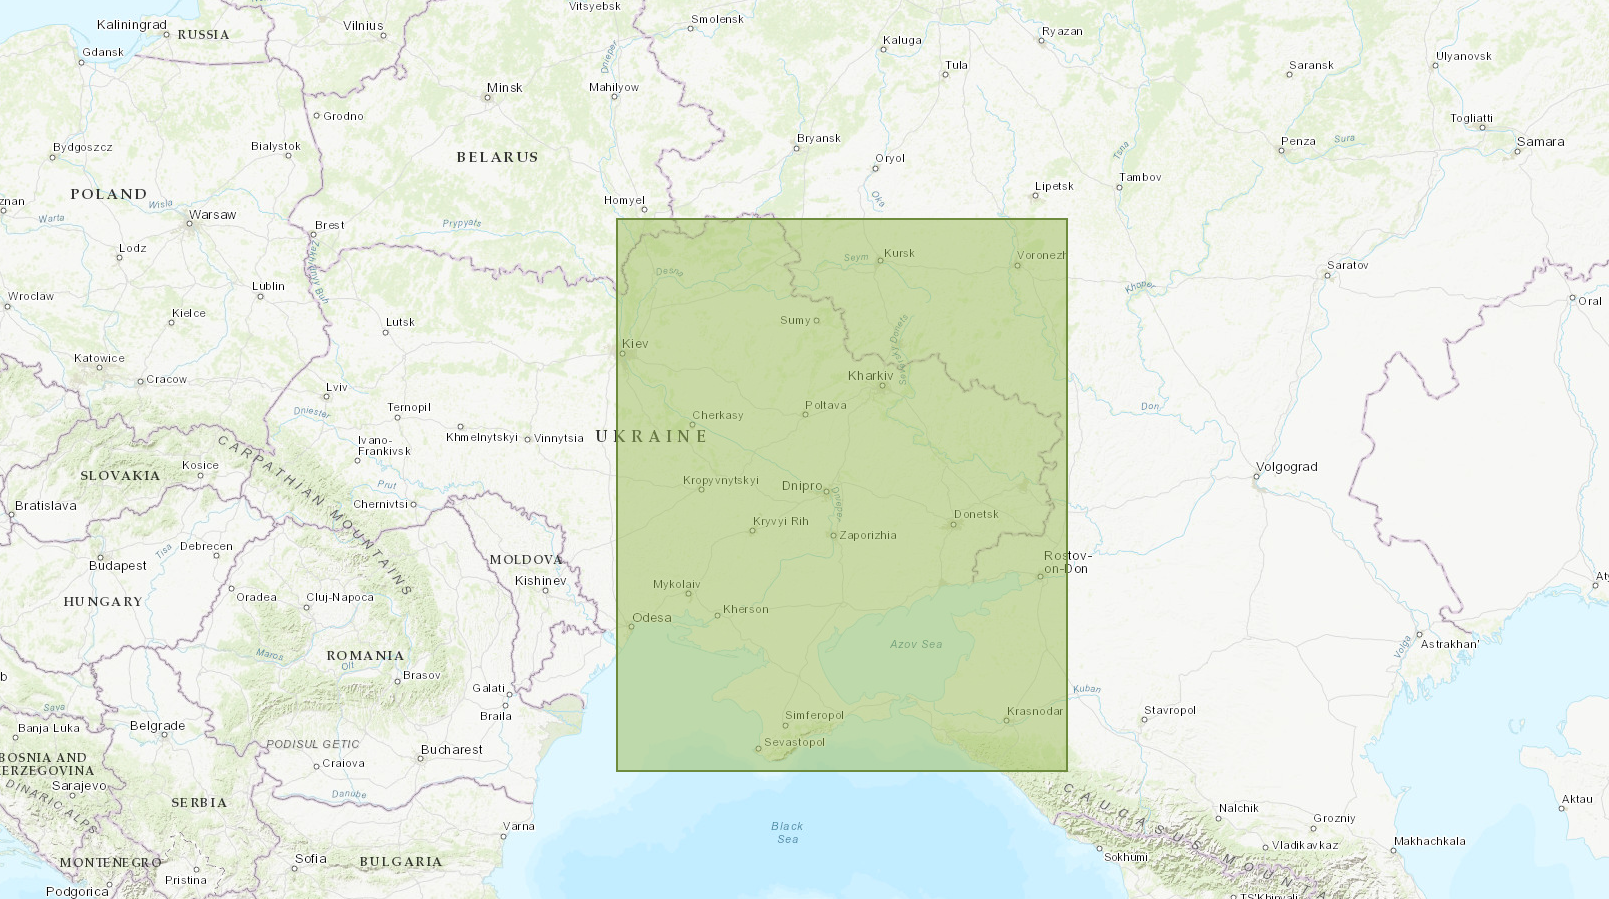
\includegraphics[width=0.8\textwidth]{map.png}
        \caption{Мапа з прямокутником, що показує область дослідження}
    \end{center}
\end{figure}

Основні маніпуляції над даними, включаючи їх аналіз та обробку, виконувались у форматі Dataframe з бібліотеки pandas. 
Він надає зручний інтерфейс для роботи з даними та дозволяє проводити різноманітні операції, такі як фільтрація, групування та візуалізація. 
Netcdf це формат в, якому дані початково зберігались і були надані з джерел.


\section{Інструменти}

Для обробки даних використовувалась мова програмування Python на веб-інтерактивній обчислювальній платформі Jupyter Notebook. 
Ця платформа була обрана через можливість поетапного виконання коду з отриманням проміжних результатів без необхідності чекати завершення роботи всієї програми. 
Це забезпечує зручність та ефективність в аналізі даних, дозволяючи швидко вносити зміни та отримувати зворотній зв'язок.

Для аналізу, візуалізації та обробки даних були використані такі бібліотеки:

\begin{itemize}
    \item NETCDF4 - Ця бібліотека була використана для роботи з NETCDF файлами, що дозволило зручно завантажувати, зберігати та обробляти великі об'єми багатовимірних даних.
    \item numpy - Використовувалася для роботи з масивами даних, забезпечуючи ефективне виконання операцій над ними, включаючи обчислення та трансформацію даних.
    \item matplotlib - Використовувалася для візуалізації даних, дозволяючи створювати різноманітні графіки та діаграми, які допомагають візуально представляти результати аналізу.
    \item pandas - Ця бібліотека була застосована для збереження даних у форматі Dataframe, що забезпечує зручний доступ до даних, їх фільтрацію, агрегацію та інші операції під час аналізу.
    \item seaborn - Використовувалась для побудови деяких графіків та дозволила виявити деякі взаємозв’язки та патерни в даних.
\end{itemize}

\section{Вигляд, паттерни та зв'язок даних}

\subsection{Дані забруднення}

Для того, щоб краще зрозуміти структуру та розподіл даних, перш ніж застосовувати методи моделювання, доцільно провести пропередній аналіз. 
Одним із важливих інструментів для цього є візуалізація даних у формі гістограми. 
Гістограма дозволить оцінити розподіл значень параметрів та прогнозованих величин.
Гістограма - це тип діаграми, яка показує частоту розподілу даних. 
Додаткові причини застосування гістограми - виявити аномалії, що мають малу частоту і мають значення сильно відмінні від основного масиву,  вони часто сильно впливають на результати застосуваня лінійної регресії і інших методів моделювання, розуміння структури даних, які впливають на вибір методу моделювання та його ефективність.


\begin{figure}[h]
    \begin{center}
        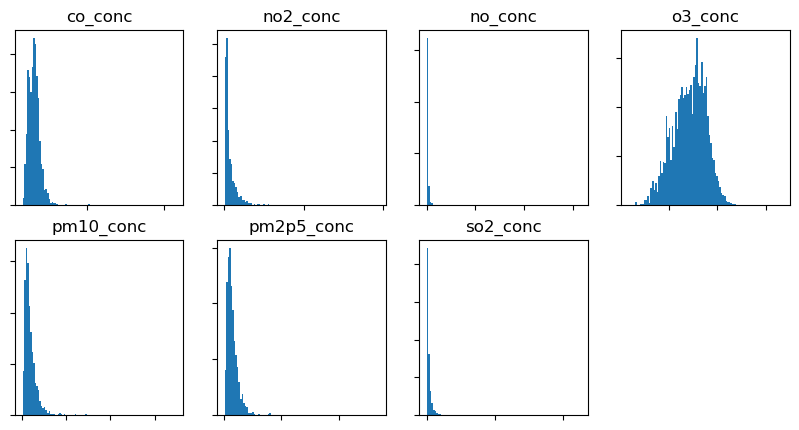
\includegraphics[width=0.8\textwidth]{rew_data_hist.png}
        \caption{Гістограми для даних про викиди}
    \end{center}
\end{figure}

На гістограмі, зображеній на рис. 2.2, можна чітко побачити, що лише дані, які стосуються викидів озону, мають розподіл, подібний до нормального. 
Це означає, що для більшості рівнів озону спостерігається концентрація значень навколо середнього, зі зменшенням частоти як для значень, що перевищують середнє, так і для тих, що знаходяться нижче середнього - гарні умови до застосування лінійної регресії.


Інші гістограми демонструють наявність аномалій, що ускладнює оцінку типів розподілів. 
Для вибору кращого діапазону застосування гістограми, що має меншу кількість аномалій, але не відкидає багато даних, доцільно розглянути діапазон значень цих параметрів. 


\begin{figure}[H]
    \begin{center}
        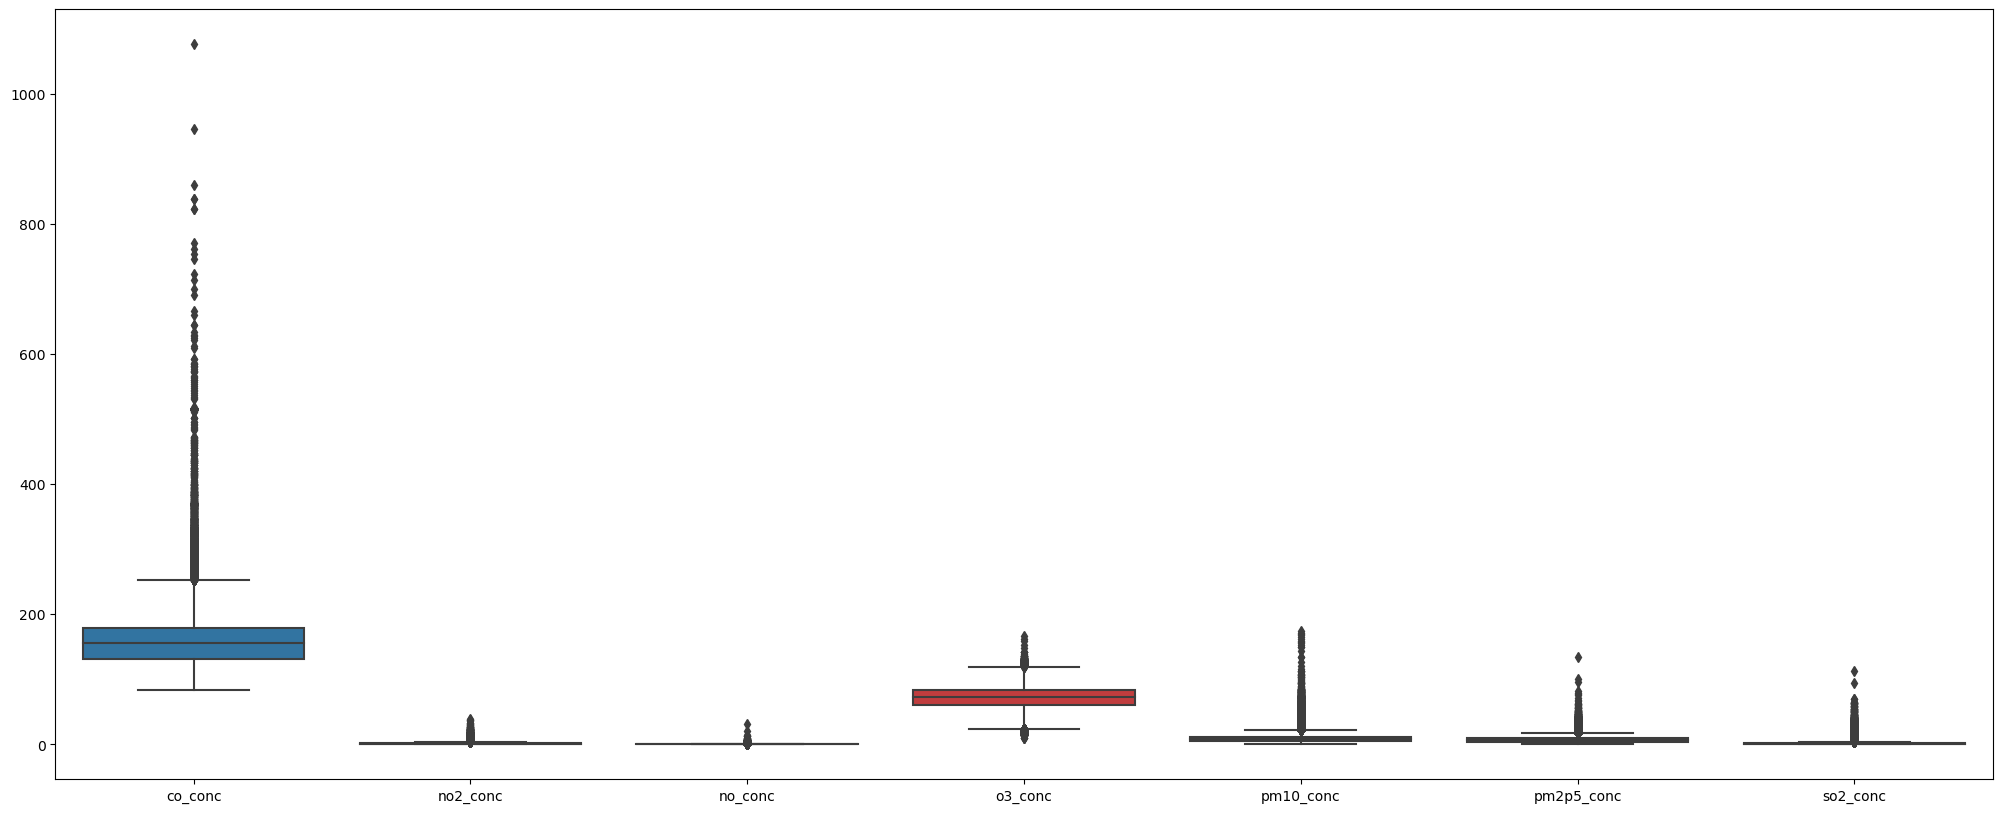
\includegraphics[width=0.8\textwidth]{range_of_data.png}
        \caption{Діапазон даних про викиди}
    \end{center}
\end{figure}


Для застосування гістограми візьмемо такі проміжки: [100; 450], [0; 8], [0; 1], [0; 130], [0; 50], [0; 25], [0; 10]. Розглянемо на прикладі моноксиду азоту і сірчастого газу, оскільки їхні гістограми були найменш ілюстративними. Максимуми по викидам цих типів становлять 31 і 112 відповідно. При цьому лише 1.5\% записів відносно моноксиду азоту більші за 1, і лише 1.2\% записів про сірчастий газ більші за 10.

Ці низькі частоти вказують на наявність аномалій, які значно впливають на загальне сприйняття розподілу даних. Тому для більш точного аналізу і візуалізації доцільно зосередитися на меншому діапазоні значень.

Вибір зазначених проміжків дозволяє краще побачити основні тенденції в розподілі даних, уникнувши впливу крайніх значень. Такий підхід допоможе виявити більш загальні патерни та забезпечить коректніше використання методів моделювання. Зокрема, гістограми з обраними діапазонами покажуть, як основна маса даних розподілена навколо середніх значень, що сприятиме точнішій оцінці можливостей застосування лінійної регресії та інших методів аналізу.

\begin{figure}[H]
    \begin{center}
        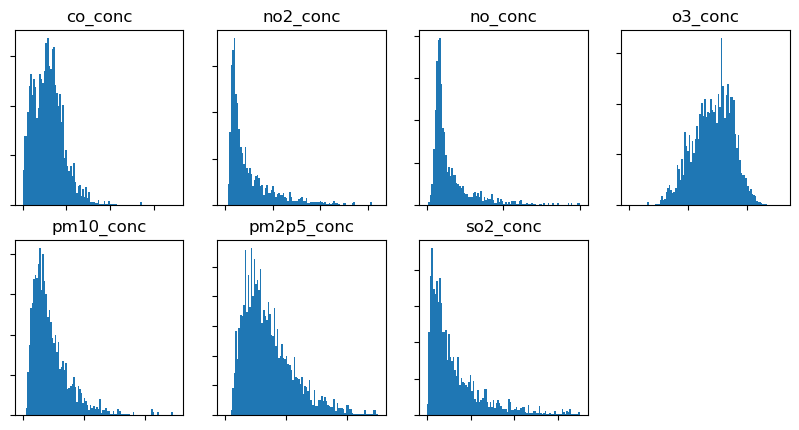
\includegraphics[width=0.8\textwidth]{scaled_histograms.png}
        \caption{Гістограми на зменшених проміжках}
    \end{center}
\end{figure}

Як видно з гістограм, дані відносно всіх викидів, окрім озону та вуглекислого газу, утворюють правосторонні розподіли. Це означає, що більшість значень зосереджені у нижньому діапазоні, з поступовим зменшенням частоти у напрямку до вищих значень. Такий тип розподілу свідчить про наявність великої кількості малих значень та кількох значно більших, що є характерним для багатьох видів забруднюючих речовин.

Варто зазначити, що вуглекислий газ не демонструє чіткого розподілу. 
Хоч його дані розміщені не симетрично вони розподілені достатньо рівномірно відносно середнього значення для можливості застосування логістичної регресії.

\subsection{Параметри прогнозування}

Для застосування моделей з розділу 3 важливо проаналізувати зв’язки між параметрами прогнозування. 
Аналіз кореляційних коефіцієнтів дозволяє виявити, які параметри мають сильний або слабкий взаємозв’язок, що може суттєво вплинути на точність та ефективність моделі. 
Високий кореляційний коефіцієнт (наближений до 1 або -1) свідчить про сильний зв’язок між параметрами, тоді як низький коефіцієнт (близький до 0) вказує на слабкий або відсутній зв’язок. 
Важливо зазначити, що даний коефіцієнт показує лише кореляцію, тобто лінійну залежність між змінними. 
Це означає, що кореляційний коефіцієнт не відображає нелінійні зв’язки, які можуть бути присутніми в даних.
Попарні кореляційні коефіцієнти наведені в таблиці:


\begin{center}
    \scalebox{0.6}{
    \begin{tabular}{|c | c| c| c| c| c| c| c| c|}
        \hline
          & SFC SW DWN	& WD10M	& WS50M	& QV2M	& WD50M	& PS	& WS10M	& T2M \\
        \hline
        SFC SW DWN	& 1.000000	& -0.185005	& -0.367893	& 0.648201 &	-0.186386 &	0.120202 &	-0.338364 &	0.641930 \\
        \hline
        WD10M	& -0.185005 &	1.000000 &	0.064822 &	-0.205908 &	0.999572 &	-0.179114 &	0.033519 &	-0.196132 \\
        \hline
        WS50M &	-0.367893 &	0.064822 &	1.000000 &	-0.211465 &	0.063771 &	0.000431 &	0.961444 &	-0.208328 \\
        \hline
        QV2M &	0.648201 &	-0.205908 &	-0.211465 &	1.000000 &	-0.206943 &	0.166831 &	-0.130927 &	0.922823 \\
        \hline
        WD50M &	-0.186386 &	0.999572 &	0.063771 &	-0.206943 &	1.000000 &	-0.179502 &	0.032133 &	-0.196800 \\
        \hline
        PS &	0.120202 &	-0.179114 &	0.000431 &	0.166831 &	-0.179502 &	1.000000 &	0.217696 &	0.280368 \\
        \hline
        WS10M &	-0.338364 &	0.033519 &	0.961444 &	-0.130927 &	0.032133 &	0.217696 &	1.000000 &	-0.106707 \\
        \hline
        T2M &	0.641930 &	-0.196132 &	-0.208328 &	0.922823 &	-0.196800 &	0.280368 &	-0.106707 &	1.000000       \\  
        \hline
    \end{tabular}}
 
    \vspace{1cm}
    \labelformat{2}{}{Таблиця 2.2: Коефіцієнти кореляції між параметрами прогнозування}
\end{center}
 
Як видно з таблиці 2.2, проблемою є лише велика кореляція між параметрами вітру на висоті 10 та 50 метрів. 
З причин, пояснених у розділі 3, ми відкидаємо одну з цих висот. 
Надалі будуть розглядатися дані лише відносно висоти 10 метрів.

Розглянемо гістограми для параметрів прогнозування, щоб детально проаналізувати розподіл значень і виявити можливі аномалії або тенденції в даних.

\begin{figure}[H]
    \begin{center}
        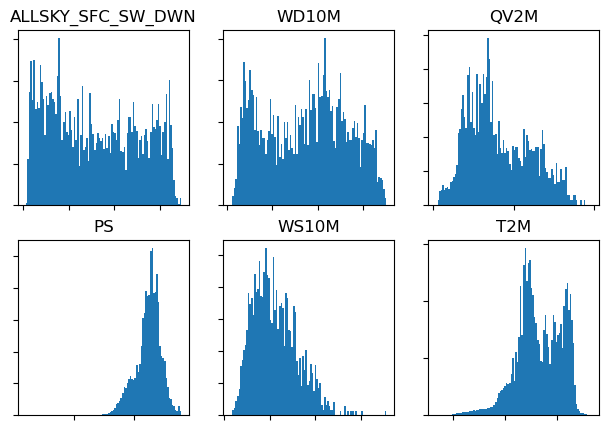
\includegraphics[width=0.6\textwidth]{climate_data_hist.png}
        \caption{Гістограми кліматичних параметрів}
    \end{center}
\end{figure}


Швидкість вітру на висоті 10 метрів та тиск мають розподіли, наближені до нормального. 
Це сприяє більш точному аналізу та застосуванню статистичних методів, що передбачають нормальність розподілу.

Інші параметри не належать до жодного з типів розподілу.

\section{Перетворення даних}

Як було описано в попередньому підрозділі, більшість прогнозованих величин не мають нормального розподілу. 
Це може ускладнити подальший аналіз та моделювання. 
Однак, за допомогою логарифмування, можна виправити цю ситуацію та наблизити розподіл даних до нормального.
Для цього ми застосуємо логарифмічне перетворення у вигляді $ln(1 + x)$, що дозволяє уникнути великих негативних величин і забезпечити коректне оброблення даних з нульовими або малими значеннями. 
Це перетворення допоможе зменшити вплив аномалій та зробити дані більш придатними для аналізу.

Таким чином, після застосування логарифмічного перетворення, розподіли викидів вуглекислого газу, твердих часток PM10 та PM2.5 стали більш наближеними до нормального. Це сприяє більш точному та надійному аналізу даних.

Проте, розподіл озону став менш подібним до нормального після застосування логарифма. 

\begin{figure}[H]
    \begin{center}
        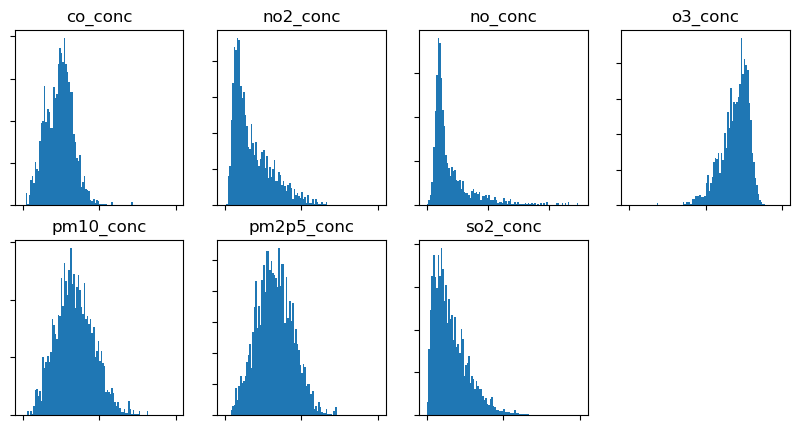
\includegraphics[width=0.8\textwidth]{log.png}
        \caption{Гістограми данних, до яких застосувалося логарифмічне перетворення}
    \end{center}
\end{figure}


Отже, використання логарифмічного перетворення для даних озону не має сенсу, оскільки це не покращує його розподіл і лише ускладнює подальший аналіз.

Далі ми застосовуємо нормалізацію даних, що приводить всі параметри та прогнозовані величини до розподілу на проміжку [0, 1]. 
Це дозволяє усунути масштабні відмінності між параметрами, забезпечуючи більш стабільну роботу алгоритмів моделювання, але трохи ускладнює інтерпретацію результатів.
Нормалізація відбувається за формулою $\frac{X- X_{min}}{X_{max} - X_{min}}$.